\everymath{\displaystyle}
\documentclass{beamer}
% \documentclass[handout]{beamer}

%\usepackage[pdftex]{color,graphicx}
\usepackage{amsmath,amssymb,amsfonts}

\mode<presentation>
{
  % \usetheme{Darmstadt}
  % \usetheme[hideothersubsections]{Hannover}
  % \usetheme[hideothersubsections]{Goettingen}
  \usetheme[hideothersubsections, right]{Berkeley}

  \usecolortheme{seahorse}
  % \usecolortheme{dolphin}
  \usecolortheme{rose}
  % \usecolortheme{orchid}

  \useinnertheme[shadow]{rounded}

  \setbeamercovered{transparent}
  % or whatever (possibly just delete it)
}

\mode<handout>{
  \setbeamercolor{background canvas}{bg=black!5}
  \usepackage{pgfpages}
  \pgfpagesuselayout{4 on 1}[a4paper,border shrink=5mm, landscape]
}

\usepackage[brazilian]{babel}
% or whatever

% \usepackage[latin1]{inputenc}
\usepackage[utf8]{inputenc}
% or whatever

\usepackage{times}
%\usepackage[T1]{fontenc}
% Or whatever. Note that the encoding and the font should match. If T1
% does not look nice, try deleting the line with the fontenc.


\title%[] % (optional, use only with long paper titles)
{Etapas da Pesquisa}

\subtitle
{Planejamento e eventuais fracassos} % (optional)

\author%[] % (optional, use only with lots of authors)
{Felipe Figueiredo}% \and S.~Another\inst{2}}
% - Use the \inst{?} command only if the authors have different
%   affiliation.

\institute[] % (optional, but mostly needed)
{
}
  % \inst{1}%
  % Department of Computer Science\\
  % University of Somewhere
  % \and
  % \inst{2}%
  % Department of Theoretical Philosophy\\
  % University of Elsewhere}
% - Use the \inst command only if there are several affiliations.
% - Keep it simple, no one is interested in your street address.

\date%[] % (optional)
{}

% \subject{Talks}
% This is only inserted into the PDF information catalog. Can be left
% out. 



% If you have a file called "university-logo-filename.xxx", where xxx
% is a graphic format that can be processed by latex or pdflatex,
% resp., then you can add a logo as follows:

\pgfdeclareimage[height=1.6cm]{university-logo}{../logo}
\logo{\pgfuseimage{university-logo}}



% Delete this, if you do not want the table of contents to pop up at
% the beginning of each subsection:
\AtBeginSubsection[]
%\AtBeginSection[]
{
  \begin{frame}<beamer>{Sumário}
    \tableofcontents[currentsection,currentsubsection]
  \end{frame}
}


% If you wish to uncover everything in a step-wise fashion, uncomment
% the following command: 

% \beamerdefaultoverlayspecification{<+->}


\begin{document}

\begin{frame}
  \titlepage
\end{frame}

\begin{frame}{Sumário}
  \tableofcontents
  % You might wish to add the option [pausesections]
\end{frame}


%% Template
% \section{}

% \subsection{}

% \begin{frame}{}
%   \begin{itemize}
%   \item 
%   \end{itemize}
% \end{frame}

% \begin{frame}
%   \begin{columns}
%     \begin{column}{5cm}
%     \end{column}
%     \begin{column}{5cm}
%     \end{column}
%   \end{columns}
% \end{frame}

% \begin{frame}{}
%   \includegraphics[height=0.4\textheight]{file1}
%   \includegraphics[height=0.4\textheight]{file2}
%   \includegraphics[height=0.4\textheight]{file3}
%   \begin{figure}
%     \caption{}
%   \end{figure}
% \end{frame}

% \begin{frame}{}
%   \begin{definition}
%   \end{definition}
%   \begin{example}
%   \end{example}
%   \begin{block}{Exercício}
%   \end{block}
% \end{frame}

\section{Planejamento da Pesquisa}

\subsection{Fases da Pesquisa}

\begin{frame}
  Tipicamente uma pesquisa se desenvolve em algumas etapas ou fases
  \begin{enumerate}
  \item Fase decisória
  \item Fase construtiva
  \item Fase redacional
  \end{enumerate}
\end{frame}

\begin{frame}{Fase decisória}
  \begin{itemize}
  \item Escolha do tema
  \item Definição e delimitação do problema de pesquisa
  \end{itemize}
\end{frame}

\begin{frame}{Fase construtiva}
  \begin{itemize}
  \item Construção de um plano de pesquisa
  \item Execução da pesquisa propriamente dita
  \end{itemize}
\end{frame}

\begin{frame}{Fase redacional}
  \begin{itemize}
  \item Análise dos dados
  \item Organização das idéias
  \item Elaboração de um relatório da pesquisa (artigo, dissertação,
    tese, etc)
  \end{itemize}
\end{frame}

\subsection{Planejamento da Pesquisa}

\begin{frame}{Formulação e planejamento}
  \begin{itemize}
  \item Escolha do assunto
  \item Levantamento do material bibliográfico
  \item Elaboração do problema de pesquisa
  \item Delimitação das questões
  \item Investigação da literatura (resumos)
  \item Obtenção do material bibliográfico necessário (artigos e livros)
  \end{itemize}
  De: Prodanov, 2013
\end{frame}

\begin{frame}{Delimitação do tema}
  \begin{block}{}
    Definir é limitar.

    \bigskip
    {\bf Oscar Wilde} ({\em O Retrato de Dorian Gray})
  \end{block}
  \begin{itemize}
  \item Área de interesse $>$ Tema $>$ Problema
  \item ``O que pretendo abordar?''
  \item Objetivos limitados e claramente definidos
  \item Explicitar a importância do tema
  \end{itemize}
\end{frame}

\begin{frame}{Tema}
  \begin{block}{}
    A importância do tema deve ser explicitada pelo pesquisador. É ele
    quem decide por que vai conduzir o trabalho a um rumo e não a
    outro. O pesquisador deverá explicitar por que o fez e por que foi
    importante e/ou estratégico fazê-lo. Ele é o autor e, portanto,
    deve saber defendê-lo.
  \end{block}
  Prodanov, 2013
\end{frame}

\begin{frame}{Escolha do tema}
  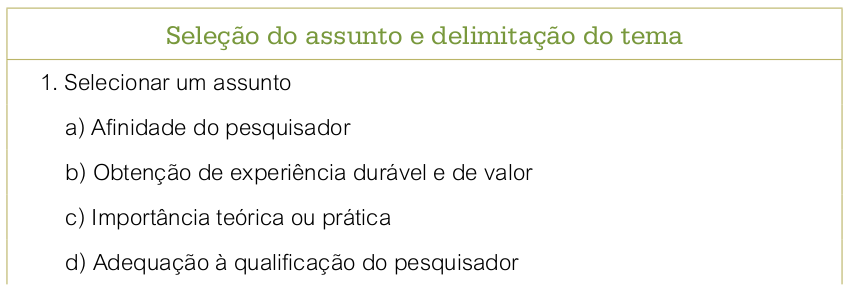
\includegraphics[width=\textwidth]{Etapas/delimitacao1}

  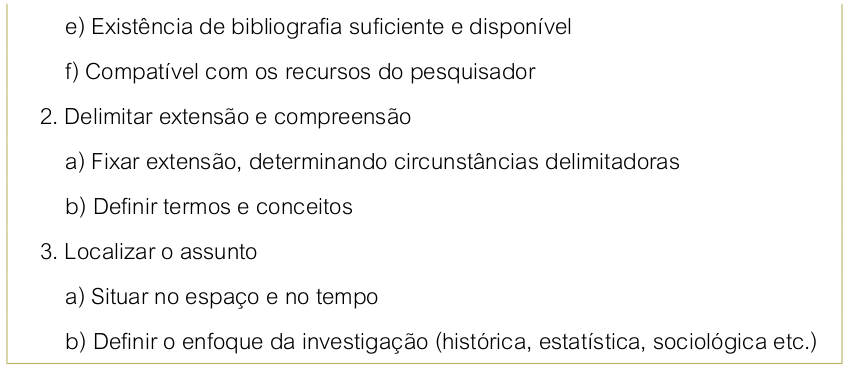
\includegraphics[width=\textwidth]{Etapas/delimitacao2}
\end{frame}

\subsection{Critérios de inclusão e exclusão}

\begin{frame}{Critérios de inclusão e exclusão}
  \begin{itemize}
  \item Validade de estudos clínicos pode ser reduzida quando
    \begin{itemize}
    \item dificuldade de comparecimento dos participantes ao centro
    \item falta de adesão do participante
    \item ausência do TCLE
    \item randomização inadequada... etc
    \end{itemize}
  \item Determinação rigorosa: um dos principais desafios para a generalização dos resultados
  \item Inclusão: determina a população sobre a qual o estudo tenta extrapolar
  \item Exclusão: cuidadosamente justificada
  \end{itemize}

  \vfill
  \small
  Fonte: JAMA 2007
\end{frame}

\begin{frame}{Critérios de inclusão e exclusão}
  \begin{block}{Critério de inclusão}
    {\em Inclusion criteria were defined as criteria governing entry or
    recruitment of individuals into the trial and describing the
    medical condition of interest.}
  \end{block}
  \begin{block}{Critério de exclusão}
    {\em All other criteria limiting the eligibility of individuals were
    treated as exclusion criteria.}
  \end{block}

  \vfill
  \small
  Fonte: JAMA 2007
\end{frame}

\begin{frame}{Critérios de exclusão}
  \begin{block}{Razões fortemente justificáveis}
    \small
    \begin{itemize}
    \item Indivíduo não assinou o TCLE
    \item Intervenção ou placebo potencialmente prejudicial
    \item Efeito da intervenção difícil de interpretar
      % \begin{itemize}
      % \item indivíduo não deve conter a característica de interesse
      % \item ... não está em risco do desfecho
      % \item ... tem alguma condição que torna o tratamento ineficaz
      % \end{itemize}
    \end{itemize}
  \end{block}
  \pause
  % podem introduzir viés
  \begin{block}{Razões difíceis de justificar}
    \small
    \begin{itemize}
    \item Idade, gênero, cond. gênero-específicas (gravidez, lactação), etnia, religião, etc. que não seja crucial para a intervenção/condição/resulta
      % Qualquer critério que não seja crucial para a intervenção/condição/resulta
    \end{itemize}
  \end{block}
  \pause
  \begin{block}{Razões potencialmente justificáveis}
    \small
    \begin{itemize}
    \item Nenhum dos dois casos anteriores
    \item Indivíduo não aderiu ao protocolo/intervenção ou faltou ao follow-up
    % \item Indivíduo falta ao follow-up
    \end{itemize}
  \end{block}

  \vfill
  \small
  Fonte: JAMA 2007
\end{frame}

\begin{frame}{Versão completa}
  \begin{center}
    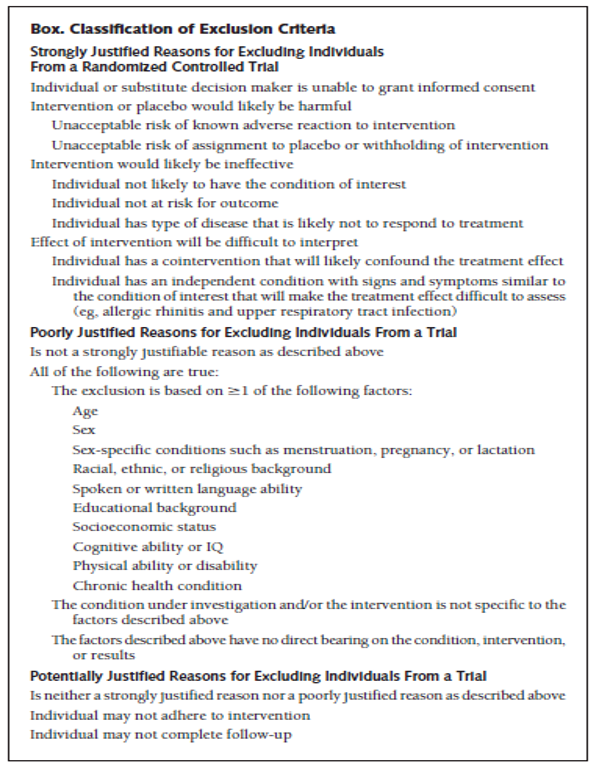
\includegraphics[height=.9\textheight]{Etapas/box-crit-exclusao}
  \end{center}
  \small
  Fonte: JAMA 2007
\end{frame}

\subsection{Metas e Cronograma}

\begin{frame}{Metas}
  
\includegraphics[width=\textwidth]{Etapas/metas}
\end{frame}

\begin{frame}{Metas}
  \begin{itemize}
  \item Definir tarefas pontuais, e seus respectivos prazos
  \item Organizar previamente as tarefas a ser concluídas
  \item (Tentar) antecipar quanto tempo levará em cada uma delas
  \end{itemize}
\end{frame}

\begin{frame}{Pequeno...}
  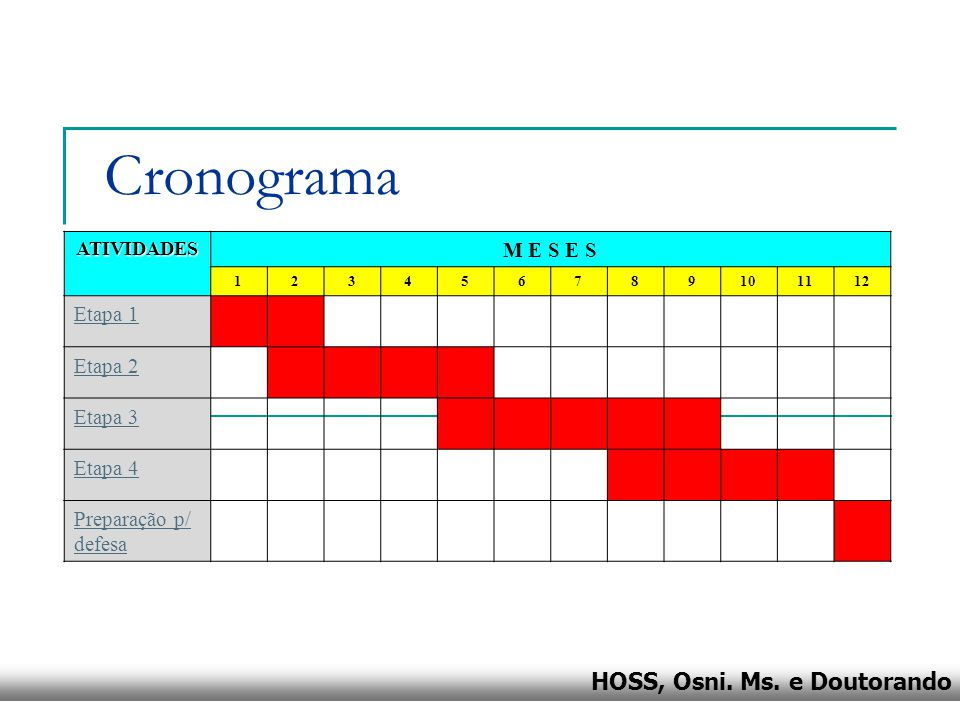
\includegraphics[width=\textwidth]{Etapas/cronograma-1}
\end{frame}

\begin{frame}{Médio...}
  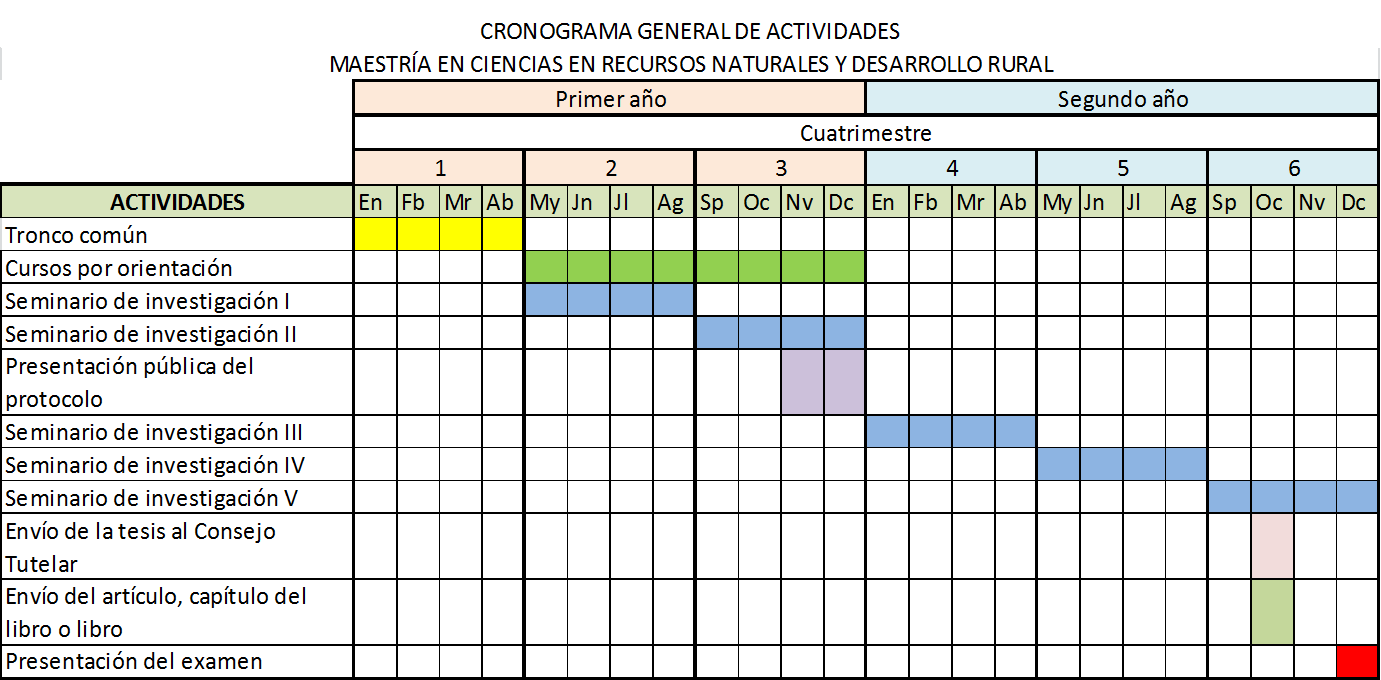
\includegraphics[width=\textwidth]{Etapas/cronograma-2}
\end{frame}

\begin{frame}{Grande...}
  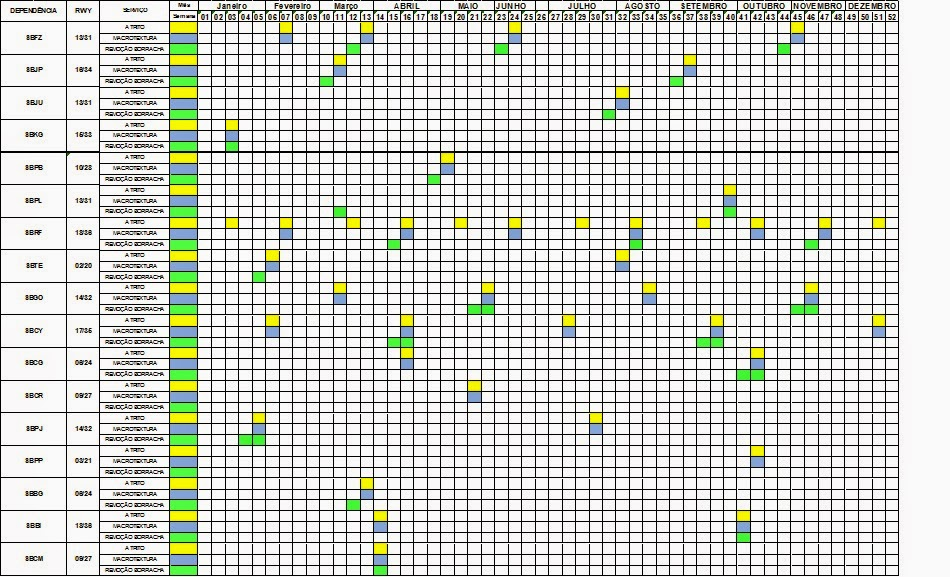
\includegraphics[width=\textwidth]{Etapas/cronograma-3}
\end{frame}

% \subsection{Execução da Pesquisa}

% \subsection{Relatório da Pesquisa}

\subsection{Execução e Relatório}

\begin{frame}{Coleta dos dados}
  \begin{itemize}
  \item Amostragem
  \item Experimentação
  \item Questionários
  \item Experimentos controlados
  \item Simples cego x duplo cego
  \end{itemize}
\end{frame}

\begin{frame}{Elaboração dos dados}
  \begin{itemize}
  \item Seleção
  \item Codificação
  \item Tabulação
  \end{itemize}
\end{frame}

\begin{frame}{Análise e interpretação dos dados}
  \begin{itemize}
  \item Análise
    \begin{itemize}
    \item Interpretação: relações entre as variáveis dependente e
      independente
    \item Explicação: esclarecimento sobre a origem da variável
      dependente
    \item Especificação: até que ponto as relações entre as variáveis
      independente e dependente são válidas (como, onde e quando).
    \end{itemize}
  \item Interpretação
    \begin{itemize}
    \item Construção de tipos, modelos esquemas
    \item Ligação com a teoria
    \end{itemize}
  \end{itemize}
  De: Lakatos, 2003
\end{frame}

\begin{frame}{Problemas a evitar}
  \begin{enumerate}
  \item Confusão entre afirmações e fatos. % As afirmações devem ser
    % comprova- das, tanto quanto possível, antes de serem aceitas como
    % fatos.
  \item Incapacidade de reconhecer limitações.%  Tanto em relação ao
    % grupo quan- to pelas situações, ou seja, tamanho, capacidade de
    % representação e a pró- pria composição, que pode levar a
    % resultados falsos.
  \item Tabulação descuidada ou incompetente. % Realizada sem os
    % cuidados ne- cessários, apresentando, por isso, traços mal
    % colocados, somas equivocadas etc.
  \item Procedimentos estatísticos inadequados. % Leva a conclusões sem
    % vali- dade, em conseqüência de conhecimentos errôneos ou
    % limitações nesse campo.
  \item Erros de cálculo. % Os enganos podem ocorrer em virtude de se
    % trabalhar com um número considerável de dados e de realizarem
    % muitas operações.
  \item Defeitos de lógica.%  Falsos pressupostos podem levar a
    % analogias inadequa- das, a confusões entre relação e causa e/ou à
    % inversão de causa e efeito.
  \item Parcialidade inconsciente do investigador.%  Déixar-se envolver
    % pelo pro- blema, inclinando-se mais à omissão de resultados
    % desfavoráveis à hipótese e enfatizando mais os dados favoráveis.
  \item Falta de imaginação. % Impede a descoberta de dados
    % significativos e/ou a capacidade de generalizações, sutilezas que
    % não escapariam a um analista mais sagaz. A imaginação, a intuição
    % e a criatividade podem auxiliar o pes- quisador, quando bem
    % treinadas.
  \end{enumerate}
  De: Lakatos, 2003
\end{frame}

% \section{Buscas}

% \subsection{Google Scholar}


\section{Fracassos}

\subsection{Fracassos?}

\begin{frame}{E aí você recebe uma carta de rejeição...}
  \centering
  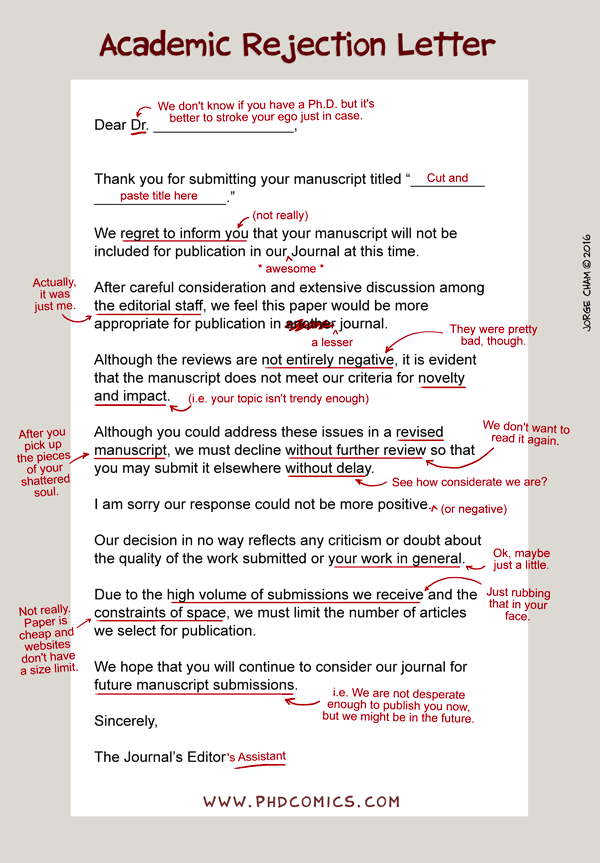
\includegraphics[height=\textheight]{Etapas/phd071316s}
\end{frame}

\begin{frame}{Rejeição}
  \begin{itemize}
  \item Diversos motivos podem levar à rejeição do texto
  \item Revisão por pares = escrutínio de todos os detalhes
  \item Análise da metodologia e argumentação
  \item Detecção de possíveis fraudes
  \item Interessante: Retraction Watch (\url{http://retractionwatch.com/})
  \end{itemize}
\end{frame}

\begin{frame}{O {\em peer review} não é perfeito}
  \begin{itemize}
  \item Somos todos humanos:
    \begin{itemize}
    \item rejeição por motivos pessoais
    \item ideologia
    \end{itemize}
  \item Falhas no processo de revisão
  \item Aceitação de estudos {\em fake}
  \item Rejeição de estudos {\em válidos}
  \end{itemize}
\end{frame}

\subsection{Notícias esdrúxulas}

\begin{frame}{Preconceito}
  Artigo rejeitado pois as autoras eram mulheres, não havia nenhum
  homem no grupo
    \begin{block}{O revisor}
      \ldots find one or two male biologists to work with (or at least
      obtain internal peer review from, but better yet as active
      co-authors), in order to serve as a possible check against
      interpretations that may sometimes be drifting too far away from
      empirical evidence into ideologically based assumptions.
    \end{block}

\url{http://retractionwatch.com/2015/04/29/its-a-mans-world-for-one-peer-reviewer-at-least/}
\end{frame}

\begin{frame}{Preconceito}
  Artigo rejeitado pois as autoras eram mulheres, não havia nenhum
  homem no grupo
    \begin{block}{A revista}
      PLOS regrets the tone, spirit and content of this particular
      review. We take peer review seriously and are diligently and
      expeditiously looking into this matter. The appeal is in
      process. PLOS allows Academic Editors autonomy in how they
      handle manuscripts, but we always follow up if concerns are
      raised at any stage of the process. Our appeals policy also
      means that any complaints of the review process can be fully
      addressed and the author given opportunity to have their paper
      re-reviewed.
    \end{block}
\end{frame}

\begin{frame}{Ou seja...}
  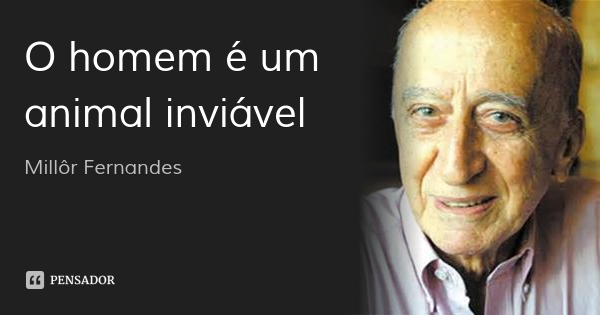
\includegraphics[width=\textwidth]{Etapas/millor}
\end{frame}

\begin{frame}{Aceitação de estudos {\em fake}}
  \begin{itemize}
  \item Caso Sokal
  \item Caso Bohannon
  \end{itemize}
\end{frame}

\begin{frame}{O caso Sokal}
  \begin{itemize}
  \item Alan Sokal (físico) publicou em 1996 um estudo na {\em Social
      Text}
  \item Criticava a qualidade dos artigos nas áreas sociais, que
    usavam indevidamente argumentos matemáticos ou físicos
  \item Submeteu um artigo que argumentava que a {\em gravidade
      quântica} tinha implicações políticas profundas
  \item Citou muitos autores reconhecidos da área, e que publicavam na
    revista
  \item Aceito para uma edição especial
  \end{itemize}
\end{frame}

\begin{frame}{O caso Sokal}
  \begin{itemize}
  \item O estudo era {\em fictício}!
  \item A argumentação era incoerente
  \item as analogias eram inválidas
  \item as citações e referências estavam fora de contexto
  \item O texto foi escrito como um {\bf trote}!
  \item Posteriormente, Sokal e Jean Bricmont publicaram um livro
    ({\em Impostures Intellectuelles}) expandindo esse tipo de crítica
    ao abuso de idéias científicas
  \end{itemize}
\end{frame}

\begin{frame}{John Bohannon}
  \begin{itemize}
  \item Em 2013 John Bohannon escreveu um artigo com sérias falhas
    metodológicas
  \item Objetivo: testar o controle de qualidade em diversas revistas
    online
  \item Resultado: 304 submissões, 157 aceites, 98 rejeitas
  \end{itemize}
  \begin{block}{}
    Any reviewer with more than a high-school knowledge of chemistry
    and the ability to understand a basic data plot should have
    spotted the paper's short-comings immediately. Its experiments are
    so hopelessly flawed that the results are meaningless.
  \end{block}
  \url{http://www.sciencemag.org/content/342/6154/60.full}
\end{frame}

\begin{frame}{Esses casos são exceção!}
  \begin{itemize}
  \item Problemas existem em qualquer aspecto da humanidade
  \item Esses casos emblemáticos são notícia (leia: raros!)
  \item O processo de {\em peer review} tradicional, embora não seja
    perfeito, é responsável pelo avanço do conhecimento nas mais
    diversas áreas do conhecimento
  \item Esse processo rejeita mais trabalhos do que aceita
  \item Como lidar com a rejeição?
  \end{itemize}
\end{frame}

\subsection{Motivos de rejeição}

\begin{frame}{8 motivos comuns para rejeição}
  \url{http://www.elsevier.com/connect/8-reasons-i-rejected-your-article}
  \begin{enumerate}
  \item<1-> Não passa pelo crivo técnico
  \item<1-> Fora do escopo
  \item<1-> Incompleto
  \item<1-> Problemas metodológicos ou de análise
  \item<1-> Conclusão não segue dos resultados
  \item<1-> Pequena extensão de artigo prévio
  \item<1-> Texto incompreensível
  \item<1-> {\em Boring}
  \end{enumerate}
\end{frame}

\begin{frame}{Crivo técnico}
  \begin{itemize}
  \item Suspeita de plágio, ou está sendo analisado por outra revista
  \item Rascunho pode faltar elementos como título, autores,
    afiliações, etc
  \item Figuras ilegíveis ou incompletas
  \item Referências podem estar incompletas, ou muito antigas
  \end{itemize}
\end{frame}

\begin{frame}{Escopo}
  \begin{itemize}
  \item Estudo pode não estar dentro do escopo ou objetivos da revista
  \item Exemplo: Para a revista {\em Carbon} o material utilizado pode
    conter carbono, mas não é carbono
  \item O estudo usa carbono, mas o foco é em algo diferente
  \item Não há inovação para a área do Carbono
  \end{itemize}
\end{frame}

\begin{frame}{Incompleto}
  \begin{itemize}
  \item O estudo contém observações, mas não é um estudo completo
  \item Discussão relaciona com descobertas de outras áreas, mas não
    todas as áreas relevantes
  \end{itemize}
\end{frame}

\begin{frame}{Metodologia ou Análise de dados}
  \begin{itemize}
  \item O procedimento não inclui um grupo controle rigorosamente
    monitorado
  \item A metodologia não é reprodutível
  \item A análise não é estatísticamente válida, ou não está de acordo
    com os padrões estabelecidos na área
  \end{itemize}
\end{frame}

\begin{frame}{{\em non sequitur}}
  As conclusões não podem ser justificadas a partir dos resultados
  \begin{itemize}
  \item Argumentos ilógicos, mal estruturados ou inválidos
  \item Os dados (evidências) não suportam as conclusões
  \item As conclusões ignoram outros resultados da literatura
  \end{itemize}
\end{frame}

\begin{frame}{Pequeno incremento}
  É apenas uma {\bf pequena} extensão de um artigo anterior,
  possivelmente pelos próprios autores
  \begin{itemize}
  \item Descobertas são um pequeno incremento, e não acrescentam ao
    conhecimento da área
  \item O artigo é visivelmente parte de um estudo maior, {\em
      picotado} na maior quantidade de artigos possível
  \end{itemize}
\end{frame}

\begin{frame}{Texto incompreensível}
  \begin{itemize}
  \item Linguagem, estrutura do texto ou figuras são problemáticas
  \item Deve-se sempre mostrar o rascunho a alguém que seja fluente ou
    nativo em Inglês.
  \end{itemize}
\end{frame}

\begin{frame}{Desinteressante}
  \begin{itemize}
  \item Apenas mostra novos dados, é incremental ou de interesse
    marginal na área
  \item A pergunta do trabalho não é do interesse da área
  \item O texto não desperta interesse do público alvo da área
  \end{itemize}
\end{frame}

\subsection{Rejeitado: e agora?}

% \begin{frame}{10 regras simples para publicar}
%   \begin{itemize}
%   \item 
%   \end{itemize}
%   \url{http://journals.plos.org/ploscollections/article?id=10.1371/journal.pcbi.0010057}
% \end{frame}

\begin{frame}{Lidando com a rejeição}
  \url{https://theihs.org/career-resources/so-they-rejected-your-paper/}

  \begin{itemize}
  \item Primeira coisa a fazer: nada. Esfrie a cabeça! (pelo menos 24-48h)
  \item Entenda os comentários dos revisores.
  \item Eles entenderam seus argumentos? Se não, por que não?
  \item Nenhum trabalho é perfeito: primeiro passo para um trabalho
    melhor
  \item Mal entendido: esclareça e ressubmeta. Bom senso: não insista!
  \end{itemize}
\end{frame}

\begin{frame}{O que fazer após a rejeição}
  \url{https://theihs.org/career-resources/what-to-do-with-your-rejected-paper/}
  \begin{itemize}
  \item Comece com uma lista de alvos para submissão.
  \item Tenha um plano B
  \item Aceite e implemente todas as sugestões e correções dos
    revisores (mesmo se for submeter para o plano B)
  \item Revisor: seu assistente de pesquisa não-remunerado
  \item Em alguns casos, as correções exigidas pelo revisor podem
    tornar seu trabalho digno de uma revista melhor que a submissão original
  \end{itemize}
\end{frame}

\begin{frame}{Humor}
  \url{http://jcs.biologists.org/content/120/8/1311.full}

  \begin{itemize}
  \item Planeje cada etapa do trabalho de correção, experimentos
    adicionais, etc
  \item Agradeça individualmente em sua carta resposta cada comentário
    e crítica de cada revisor
  \item Escreva sua resposta indicando exatamente \alert{como} atendeu
    a \alert{cada} crítica
  \item Responda a cada revisor individualmente, mesmo que
    repetitivo. Quantas vezes for necessário
  \end{itemize}
\end{frame}

\begin{frame}{Humor 2}
  
\includegraphics[width=\textwidth]{Etapas/olympus-abs}

  \url{http://arxiv.org/abs/math/0604049}
\end{frame}

\begin{frame}{Humor 2}
  \begin{block}{}
    The problem of Jacobian Conjecture is very hard. Perhaps it will
    take human being another 100 years to solve it. \alert{Your
      attempt is noble, Maybe the Gods of Olympus will smile on you
      one day.} Do not be too disappointed. B. Sagre has the honor of
    publishing three wrong proofs and C. Chevalley mistakes a wrong
    proof for a correct one in the 1950’s in his Math Review comments,
    and I.R. Shafarevich uses Jacobian Conjecture (to him it is a
    theorem) as a fact. You are in a good company. One only remembers
    the correct statements from Scientists and Mathematicians, nobody
    remembers the wrong ones.
  \end{block}
\end{frame}

\begin{frame}{Referências}
  \begin{itemize}
  \item Van Spall HG, Toren A, Kiss A, Fowler RA. Eligibility criteria of randomized controlled trials published in high-impact general medical journals: a systematic sampling review. Jama. 2007 Mar 21;297(11):1233-40.
  \end{itemize}
\end{frame}

\end{document}
